Unlike texts, humans can sense patterns in an image by seeing it. The first metrics to measure the efficacity of the algorithm is the visual analysis. \\

As an example of chaotic map, let's consider the well-known discrete logistic map defined as follow :
\begin{equation*}
	r_{n+1} = \mu r_n (1-r_n), \quad \forall n \in \mathbb{N}
\end{equation*}

\begin{figure}[!h]
\centering
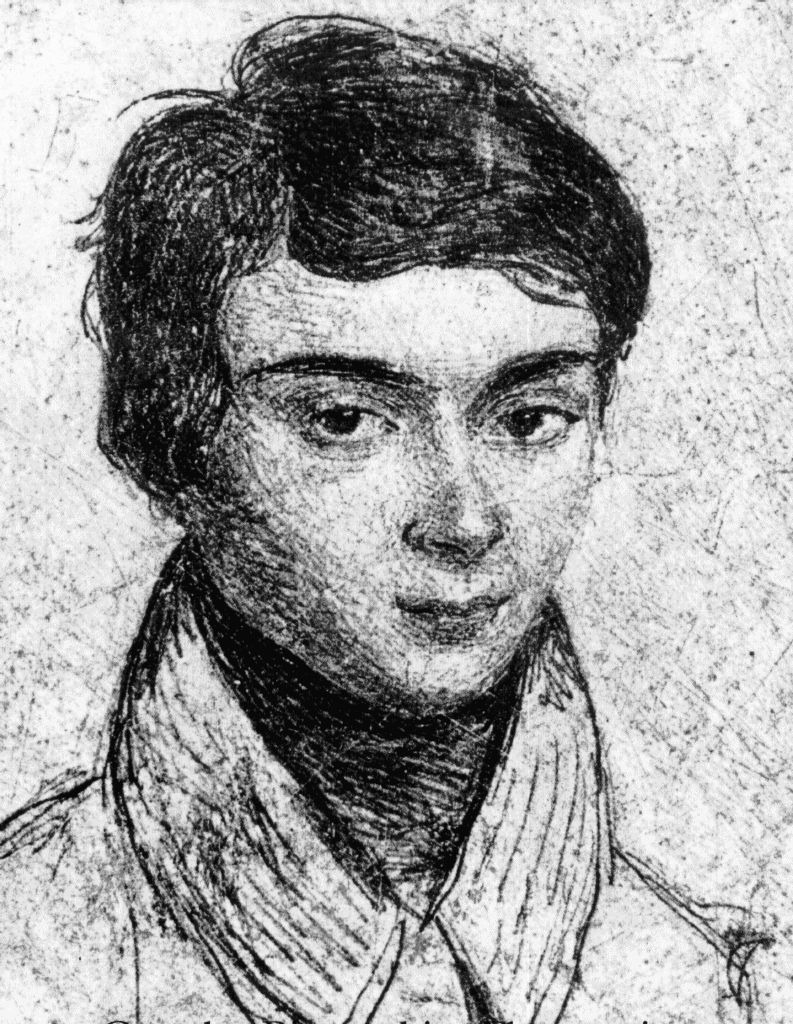
\includegraphics[scale=0.8]{tex/img/galois.jpg}
$\rightarrow$
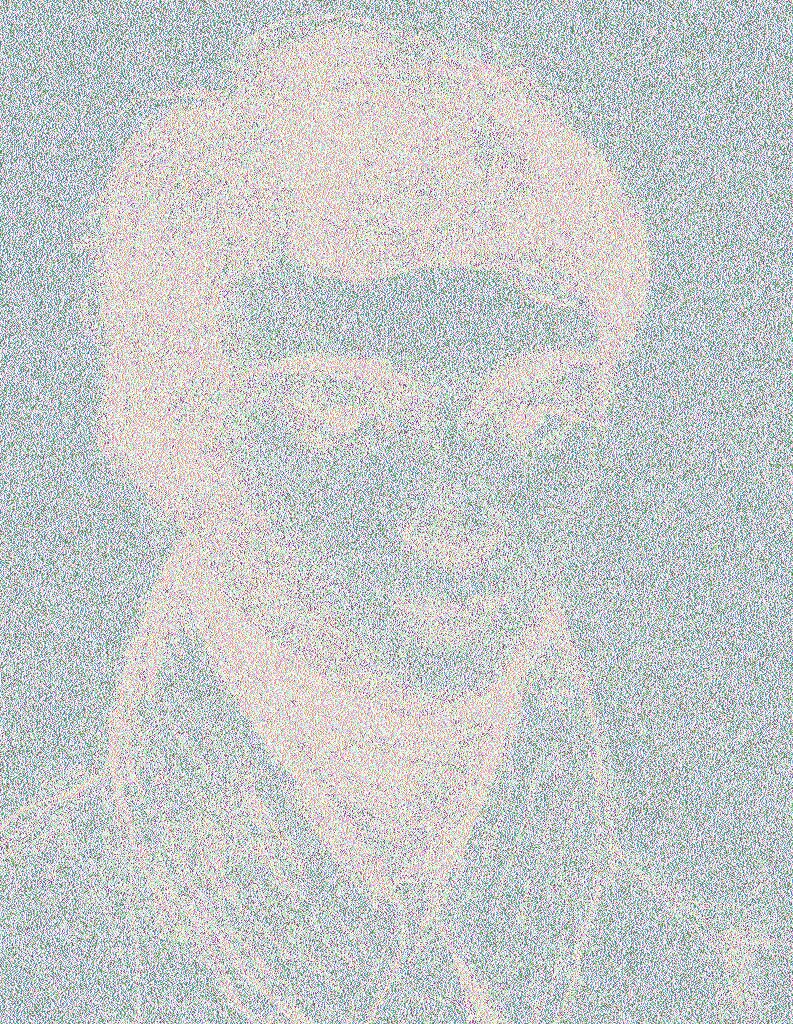
\includegraphics[scale=0.0755]{tex/img/galois1lm.jpg}
$\rightarrow$
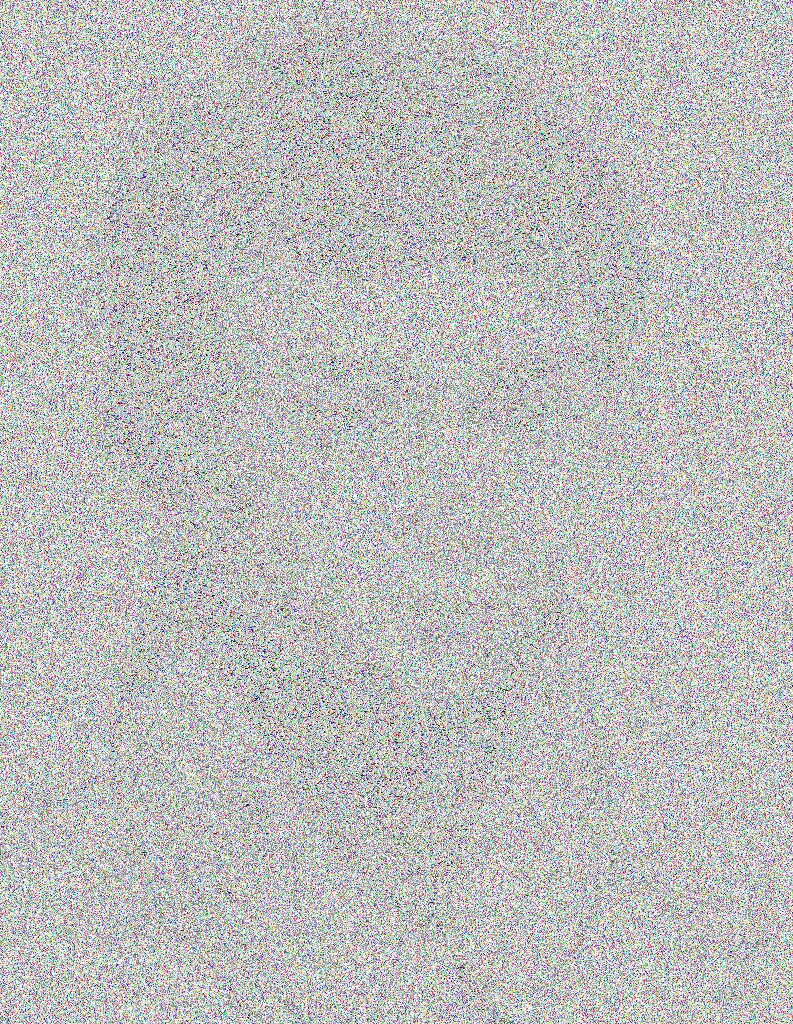
\includegraphics[scale=0.0755]{tex/img/galois2lm.jpg} \vspace{1em} \\
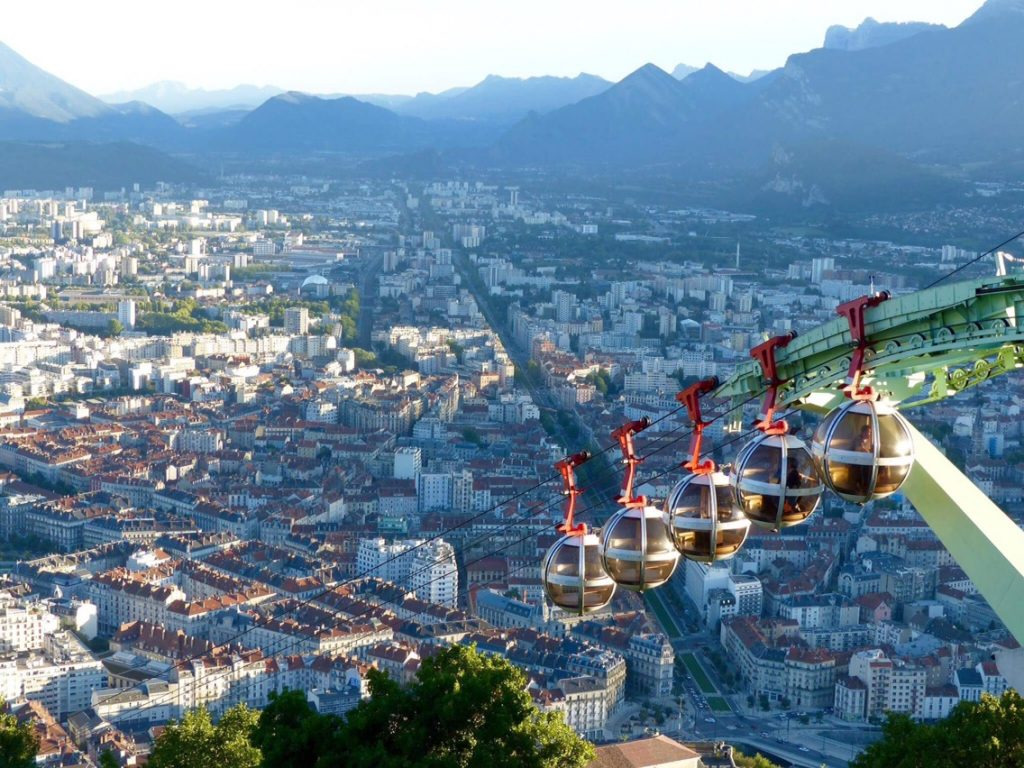
\includegraphics[scale=1.01]{tex/img/grenoble_city.jpg}
$\rightarrow$

\includegraphics[scale=0.0955]{tex/img/grenoble_city2lm.jpg}
\caption{Encryption of \textit{galois.bmp} using the logistic map ($\mu=3.89$, $r_0=0.6104$) and then using another XOR logistic map ($\mu=3.79$, $r_0=0.902$) and the encryption of \textit{grenoble\_city.bmp} with the XOR logistic map}
\end{figure}

From the results of the encryption of \textit{galois.bmp}, we can already understand a weakness of the encryption algorithm with the discrete logistic map and black and white images encoded as RGBa images. In fact, the XOR bitwise operation have the following properties, $\forall x \in \mathbb{N}$ :
\vspace{-0.4em}
\begin{align*}
	& x \oplus 0 = x \\
	& x \oplus x = 0
\end{align*}

These properties combined with the high correlation between adjacent pixels lead to some optical illusions which let a human sense the shape of the original image. Obviously, this kind of behaviour need be avoided while doing image encryption. \\
However, this behaviour tends to disappear using multiple discrete logistic maps as it is shown Figure 3. \\

\begin{figure}[!h]
\centering
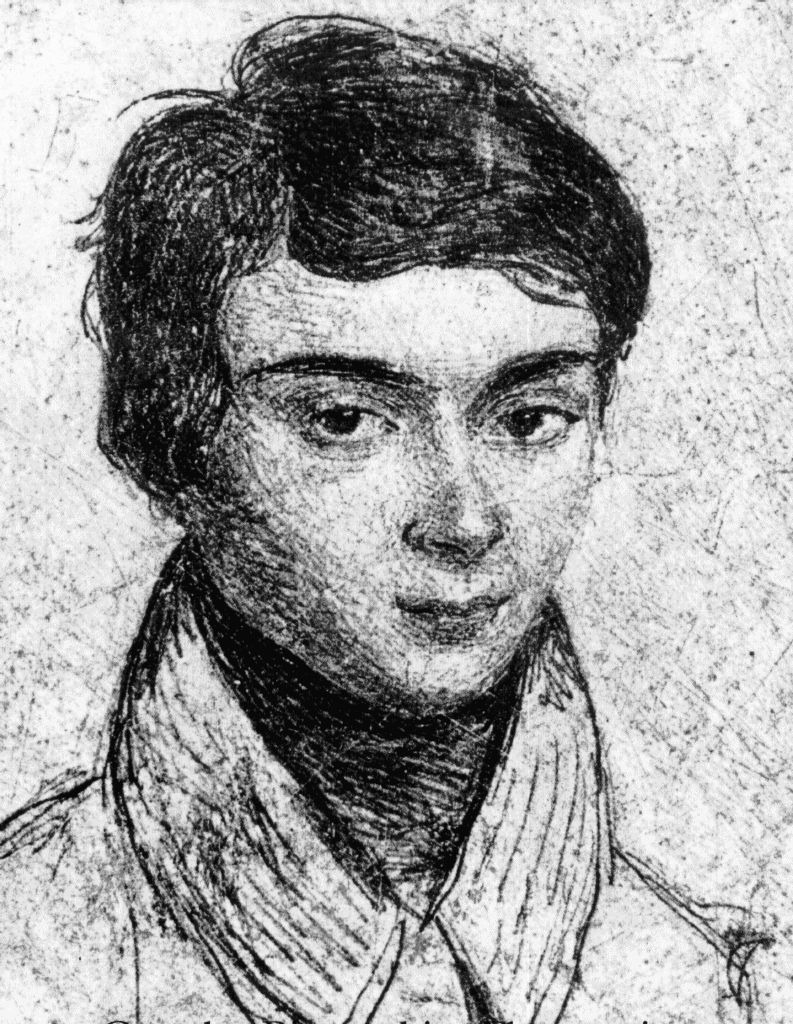
\includegraphics[scale=1.06]{tex/img/galois.jpg}
$\rightarrow$

\includegraphics[scale=0.1]{tex/img/galoismlm.jpg}
\caption{Encryption of \textit{galois.bmp} using 4 discrete logistic maps with randomly chosen parameters}
\end{figure}

Consequently, using more chaotic maps to generate the encryption key result of more computational time. Inspired by traditional encryption algorithm (AES for example), we could think for bits permutations to avoid the utilisation of multiple chaotic maps. Nonetheless, those permutations required a lot of computational time either, a real benckmarking on various size and type of images need to be done to conclude on the best way to improve the proposed algorithm.
